% =============================================================================
% Module 2: Light Deflection in Curved Spacetime
% =============================================================================
% Sources: Carroll Ch. 5.5, Congdon & Keeton Ch. 3.4 (eqs. 3.87--3.96,
%          3.97--3.110), Narayan & Bartelmann Sec. 2.1
% Mathematica: ../Mathematica/02_Light_Deflection/
% =============================================================================

\chapter{Light Deflection in Curved Spacetime}
\label{ch:light_deflection}

\begin{quote}
\textit{The chief attraction of the theory lies in its logical completeness.
If a single one of the conclusions drawn from it proves wrong, it must be
given up; to modify it without destroying the whole structure seems to be
impossible.}
\hfill --- Albert Einstein, 1919
\end{quote}

\noindent
In Module~1d we derived the effective potential for geodesic motion in
Schwarzschild spacetime, and in Module~1e we obtained the deflection
angle $\alphahat = 4\Gnewton M / (\speedoflight^2 b)$ via the
weak-field / Born approximation, showing how the factor of 2 over
Newtonian gravity arises from the equal contributions of temporal and
spatial curvature.  Now we derive this same result rigorously from the
\textit{exact} null geodesic orbit equation in the full Schwarzschild
metric.  This is
the single most important result in gravitational lensing theory --- every
lens equation, every magnification formula, and every time delay expression
ultimately rests on it.

We also derive the Shapiro time delay, which provides the second
observable consequence of light propagation through a gravitational field,
and compute the deflection for several astrophysically relevant systems:
the Sun (Eddington's 1919 test), Jupiter, and a typical galaxy lens.

\medskip
\noindent
\textbf{Companion Mathematica files:}
\begin{itemize}[nosep]
    \item \mathlink{02_Light_Deflection/deflection_angle.wl}{deflection\_angle.wl}
          --- symbolic derivation of the deflection angle integral,
          weak-field expansion, numerical evaluation for Sun/Jupiter/galaxy,
          Shapiro delay, exact vs.\ approximate comparison, and figure generation
    \item \mathlink{02_Light_Deflection/deflection_geometry.nb}{deflection\_geometry.nb}
          --- interactive notebook: ray-bending geometry, sliders for~$M$
          and~$b$, exact vs.\ weak-field comparison with error percentage
\end{itemize}


% =====================================================================
\section{Introduction: Null Geodesics and the Deflection Problem}
\label{sec:deflection_intro}

Light follows \textbf{null geodesics} in curved spacetime: paths for which
$ds^2 = 0$ at every point.  In Module~1d we showed that for a photon in
the equatorial plane of the Schwarzschild metric, the conserved energy~$E$
and angular momentum~$L$ reduce the equations of motion to a single radial
equation (cf.\ eqs.~\ref{eq:conserved_E}--\ref{eq:conserved_L} and the
null geodesic orbit equation~\eqref{eq:photon_orbit} from Module~1d):
\begin{equation}
    \frac{d\phi}{dr} = \pm \frac{L}{r^2}
    \left[\frac{E^2}{\speedoflight^2}
    - \frac{L^2}{r^2}\!\left(1 - \frac{\RS}{r}\right)
    \right]^{-1/2} ,
    \label{eq:photon_orbit_eq}
\end{equation}
where $\RS = 2\Gnewton M / \speedoflight^2$ is the Schwarzschild radius
(Congdon \& Keeton eq.~3.87).

The physical setup is as follows.  A photon approaches a mass~$M$ from
infinity, reaches a distance of closest approach~$r_0$, and then escapes
back to infinity.  The total change in the azimuthal angle~$\phi$ is
$\Delta\phi$; in flat spacetime this would be~$\pi$ (a straight line), so
the \textbf{deflection angle} is
\begin{equation}
    \alphahat = \Delta\phi - \pi \,.
    \label{eq:deflection_def}
\end{equation}
Our goal in this chapter is to evaluate $\Delta\phi$ and show that, in the
weak-field limit,
\begin{equation}
    \boxed{
    \alphahat = \frac{4\Gnewton M}{\speedoflight^2\, b}
    }
    \label{eq:alphahat_main}
\end{equation}
where $b$ is the impact parameter.  This is the fundamental result of
gravitational lensing.


% =====================================================================
\section{Soldner's Newtonian Calculation (1801)}
\label{sec:soldner}

Before Einstein, Johann Georg von Soldner (1801) computed the deflection
of light using Newtonian gravity, treating a photon as a corpuscle of
mass~$m$ traveling at speed~$\speedoflight$.

\begin{remark}
Soldner's calculation predates general relativity by over a century.
It is both historically important and pedagogically useful: it gives
exactly \textit{half} the correct GR answer, and understanding
\textit{why} illuminates the role of spatial curvature.
\end{remark}

Consider a particle approaching a mass~$M$ on a hyperbolic trajectory with
velocity~$v_\infty = \speedoflight$ at infinity.  The Newtonian equations
of motion in polar coordinates yield the orbit equation
\begin{equation}
    r(\phi) = \frac{p}{1 + e\cos\phi} \,,
    \label{eq:newtonian_orbit}
\end{equation}
where $p = L^2/(GM)$ and $e = \sqrt{1 + 2\mathcal{E}L^2/(G^2 M^2)}$ is the
eccentricity (with $\mathcal{E} = \half \speedoflight^2$ for an unbound
particle at speed~$\speedoflight$).

The asymptotic directions correspond to $r \to \infty$, i.e.,
$\cos\phi = -1/e$.  The total angle swept is $\Delta\phi = \pi + 2\delta$,
where $\sin\delta = 1/e$.  For large impact parameter ($b \gg \RS$), the
eccentricity is large and $\delta \approx 1/e \ll 1$, giving
\begin{equation}
    \alphahat_{\mathrm{Newton}} = 2\delta \approx \frac{2}{e}
    = \frac{2\Gnewton M}{\speedoflight^2\, b} \,.
    \label{eq:soldner_deflection}
\end{equation}

\begin{exercise}
\label{ex:soldner}
Derive eq.~\eqref{eq:soldner_deflection} in detail.  Start from the
Newtonian orbit equation for a massless particle with $v_\infty =
\speedoflight$ and impact parameter~$b$.
\begin{enumerate}[label=(\alph*)]
    \item Show that the semi-latus rectum is $p = b^2 \speedoflight^2 /
          (\Gnewton M)$ and the eccentricity is
          $e = \sqrt{1 + b^2 \speedoflight^4 / (\Gnewton M)^2}$.
    \item For $b \gg \Gnewton M / \speedoflight^2$, show that
          $\alphahat_{\mathrm{Newton}} = 2\Gnewton M /
          (\speedoflight^2 b)$.
\end{enumerate}
\textit{Hint:} The angular momentum is $L = b\speedoflight$ and the energy
is $\mathcal{E} = \half \speedoflight^2$.
\end{exercise}


% =====================================================================
\section{The GR Deflection Angle --- Full Derivation}
\label{sec:gr_deflection}

We now follow Congdon \& Keeton Sec.~3.4.1 (eqs.~3.87--3.96) to derive
the deflection angle in general relativity.  The result will be
$\alphahat = 4\Gnewton M / (\speedoflight^2 b)$ --- exactly \textbf{twice}
the Newtonian prediction.

\subsection{The Impact Parameter}
\label{sec:impact_parameter}

The \textbf{impact parameter} $b$ is defined as the perpendicular distance
between the undeflected ray (the asymptotic straight line at $r \to \infty$)
and the mass~$M$.  From the conserved quantities, it is related to $E$ and
$L$ by (Congdon \& Keeton eq.~3.88):
\begin{equation}
    b = \frac{\speedoflight\, L}{E} \,.
    \label{eq:impact_parameter}
\end{equation}

\subsection{Distance of Closest Approach}
\label{sec:closest_approach}

At the turning point $r = r_0$, the radial velocity vanishes:
$dr/d\lambda = 0$.  From the radial equation of motion, this gives
(Congdon \& Keeton eq.~3.90):
\begin{equation}
    \frac{E^2}{\speedoflight^2} - \frac{L^2}{r_0^2}
    \left(1 - \frac{\RS}{r_0}\right) = 0 \,.
    \label{eq:turning_point}
\end{equation}
Substituting $b = \speedoflight L / E$ and defining $m \equiv \Gnewton M /
\speedoflight^2 = \RS/2$, we obtain
\begin{equation}
    \frac{r_0^2}{b^2} = 1 - \frac{2m}{r_0} \,.
    \label{eq:r0_implicit}
\end{equation}
In the weak-field limit $m/r_0 \ll 1$, we can solve perturbatively:
$r_0 \approx b\left(1 - m/b + \cdots\right)$, so to leading order
$r_0 \approx b$.

\subsection{The Total Azimuthal Change}
\label{sec:azimuthal_integral}

By symmetry, the total angle swept from $r = \infty$ (incoming) to
$r = \infty$ (outgoing) is twice the angle from $r_0$ to infinity:
\begin{equation}
    \Delta\phi = 2 \int_{r_0}^{\infty}
    \frac{L}{r^2}
    \left[\frac{E^2}{\speedoflight^2}
    - \frac{L^2}{r^2}\!\left(1 - \frac{\RS}{r}\right)
    \right]^{-1/2} dr \,.
    \label{eq:delta_phi_integral}
\end{equation}
Substituting $b = \speedoflight L/E$ and simplifying
(Congdon \& Keeton eq.~3.91):
\begin{equation}
    \Delta\phi = 2 \int_{r_0}^{\infty}
    \frac{dr}{r^2}
    \left[\frac{1}{b^2}
    - \frac{1}{r^2}\!\left(1 - \frac{2m}{r}\right)
    \right]^{-1/2} .
    \label{eq:delta_phi_simplified}
\end{equation}

\subsection{Change of Variables}
\label{sec:substitution}

Following Congdon \& Keeton, we introduce the substitution $u = r_0 / r$
(so $u = 0$ at $r = \infty$ and $u = 1$ at $r = r_0$):
\begin{equation}
    \Delta\phi = 2 \int_0^1
    \frac{du}{\sqrt{\displaystyle
    \frac{r_0^2}{b^2} - u^2 + 2m\,\frac{u^3}{r_0}}} \,.
    \label{eq:delta_phi_u}
\end{equation}
Using eq.~\eqref{eq:r0_implicit} to replace $r_0^2/b^2 = 1 - 2m/r_0$
(Congdon \& Keeton eq.~3.93):
\begin{equation}
    \Delta\phi = 2 \int_0^1
    \frac{du}{\sqrt{\displaystyle
    (1 - u^2) - \frac{2m}{r_0}(1 - u^3)}} \,.
    \label{eq:delta_phi_u2}
\end{equation}

\subsection{Weak-Field Expansion}
\label{sec:weak_field_expansion_deflection}

We define the small parameter $\varepsilon \equiv m/r_0 \ll 1$ and expand
the integrand to first order in~$\varepsilon$.  Writing
$f(u) = (1-u^2) - 2\varepsilon(1 - u^3)$, we use
\begin{equation}
    \frac{1}{\sqrt{f}} \approx
    \frac{1}{\sqrt{1 - u^2}}
    + \frac{\varepsilon(1 - u^3)}{(1 - u^2)^{3/2}}
    + \order{\varepsilon^2} \,.
    \label{eq:integrand_expansion}
\end{equation}
Therefore (Congdon \& Keeton eq.~3.94):
\begin{equation}
    \Delta\phi \approx 2\int_0^1 \frac{du}{\sqrt{1 - u^2}}
    + 2\varepsilon \int_0^1 \frac{1 - u^3}{(1-u^2)^{3/2}}\, du
    + \order{\varepsilon^2} \,.
    \label{eq:delta_phi_expanded}
\end{equation}

\subsection{Evaluating the Integrals}
\label{sec:integral_evaluation}

\noindent\textbf{Zeroth-order integral:}  With the substitution
$u = \sin\theta$:
\begin{equation}
    I_0 = 2\int_0^1 \frac{du}{\sqrt{1 - u^2}}
    = 2\left[\arcsin u\right]_0^1 = 2 \cdot \frac{\pi}{2} = \pi \,.
    \label{eq:I0}
\end{equation}
This is the flat-spacetime result: no deflection.

\medskip
\noindent\textbf{First-order integral:}  We need
(Congdon \& Keeton eq.~3.95):
\begin{equation}
    I_1 = 2\int_0^1 \frac{1 - u^3}{(1 - u^2)^{3/2}}\, du \,.
    \label{eq:I1_def}
\end{equation}
Factor the numerator: $1 - u^3 = (1 - u)(1 + u + u^2)$ and
$1 - u^2 = (1-u)(1+u)$, so
\begin{equation}
    \frac{1 - u^3}{(1-u^2)^{3/2}}
    = \frac{(1-u)(1 + u + u^2)}{(1-u)^{3/2}(1+u)^{3/2}}
    = \frac{1 + u + u^2}{(1-u)^{1/2}(1+u)^{3/2}} \,.
    \label{eq:integrand_factored}
\end{equation}
The bare integral $\int_0^1 (1-u^3)(1-u^2)^{-3/2}\, du$ evaluates
to~$2$ (as verified in Mathematica --- see
\mathlink{02_Light_Deflection/deflection_angle.wl}{deflection\_angle.wl}),
so
\begin{equation}
    I_1 = 2 \times 2 = 4 \,.
    \label{eq:I1_result}
\end{equation}

\begin{remark}
The evaluation of $\int_0^1 (1-u^3)(1-u^2)^{-3/2}\, du = 2$ is a good
exercise in integration techniques.  One approach: split
$1 + u + u^2 = (1 + u)^2 - u$ and evaluate each piece separately via
trigonometric/hyperbolic substitution.  The Mathematica script verifies
this symbolically.
\end{remark}

\subsection{The Deflection Angle}
\label{sec:deflection_result}

Assembling the result (Congdon \& Keeton eq.~3.96): using
$\Delta\phi = I_0 + \varepsilon\, I_1 + \order{\varepsilon^2}$,
\begin{equation}
    \Delta\phi = \pi + 4\varepsilon + \order{\varepsilon^2}
    = \pi + \frac{4m}{r_0} + \order{m/r_0}^2 \,.
    \label{eq:delta_phi_result}
\end{equation}
Since $r_0 \approx b$ to leading order and $m = \Gnewton M / \speedoflight^2$:
\begin{equation}
    \boxed{
    \alphahat = \Delta\phi - \pi
    = \frac{4\Gnewton M}{\speedoflight^2\, b}
    + \order{\Gnewton M / (\speedoflight^2 b)}^2
    }
    \label{eq:alphahat_result}
\end{equation}
This is the \textbf{Einstein deflection angle} for a point mass in the
weak-field limit.

\begin{figure}[ht]
    \centering
    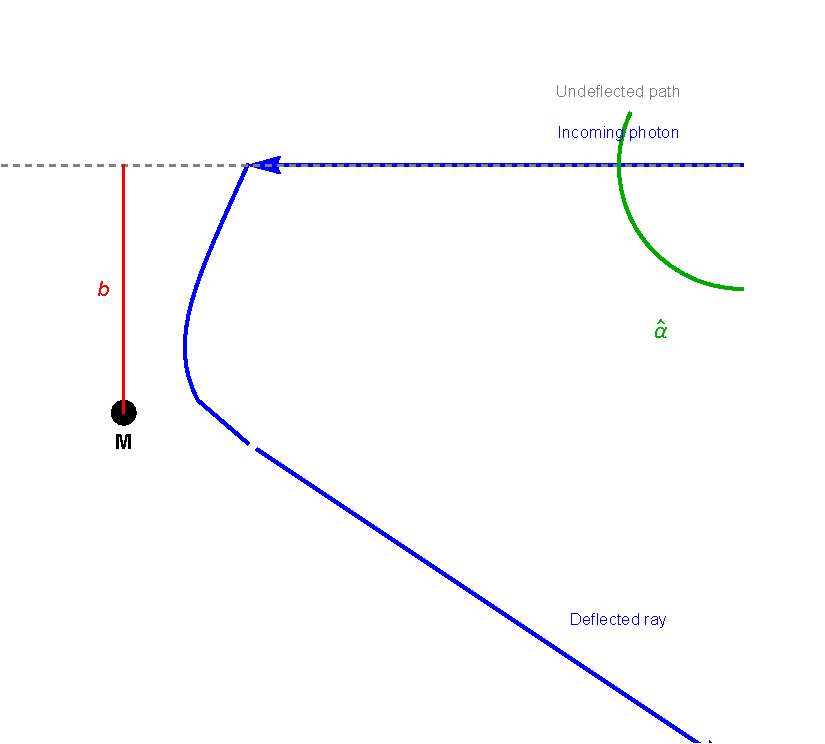
\includegraphics[width=0.75\textwidth]{../Figures/02_Light_Deflection/deflection_geometry.pdf}
    \caption{Geometry of gravitational light deflection by a point mass~$M$.
    A photon approaches from the right with impact parameter~$b$, reaches
    closest approach at~$r_0 \approx b$, and is deflected by
    $\alphahat = 4\Gnewton M/(\speedoflight^2 b)$.  The dashed line shows
    the undeflected path.  Generated by
    \texttt{deflection\_angle.wl}.}
    \label{fig:deflection_geometry}
\end{figure}

\begin{exercise}
\label{ex:gr_vs_newton}
Show that the GR deflection angle~\eqref{eq:alphahat_result} is exactly
twice the Newtonian prediction~\eqref{eq:soldner_deflection}.  Explain
physically why:
\begin{enumerate}[label=(\alph*)]
    \item The Newtonian calculation accounts for the deflection due to the
          gravitational potential (temporal curvature of the metric,
          $g_{tt}$), but ignores spatial curvature ($g_{rr}$).
    \item In GR, both $g_{tt}$ and $g_{rr}$ deviate from flat space by
          the same amount (to leading order in $m/r$), so the spatial
          curvature doubles the deflection.
\end{enumerate}
\textit{Hint:} Expand the Schwarzschild line element in isotropic
coordinates and identify the contributions from the time--time and
space--space components of the metric.
\end{exercise}


% =====================================================================
\section{The Shapiro Time Delay}
\label{sec:shapiro_delay}

In addition to deflecting light, a gravitational field \textit{slows it
down} --- or more precisely, causes an excess travel time relative to the
flat-spacetime path.  This effect was predicted by Irwin Shapiro in 1964
and first measured using radar echoes from Mercury and Venus.

Following Congdon \& Keeton Sec.~3.4.2 (eqs.~3.97--3.110), we derive the
time delay for a photon passing near a point mass.

\subsection{Coordinate Travel Time}
\label{sec:coordinate_travel_time}

For a photon on a null geodesic, we can write $dt/dr$ using the
conserved quantities (Congdon \& Keeton eq.~3.97):
\begin{equation}
    \frac{dt}{dr} = \frac{E / \speedoflight^2}{(1 - \RS/r)}
    \left[\frac{E^2}{\speedoflight^2}
    - \frac{L^2}{r^2}\left(1 - \frac{\RS}{r}\right)
    \right]^{-1/2} .
    \label{eq:dt_dr}
\end{equation}
The coordinate time for the photon to travel from closest approach $r_0$ to
a radial distance~$R$ is (Congdon \& Keeton eq.~3.98):
\begin{equation}
    T(R) = \int_{r_0}^{R} \frac{dt}{dr}\, dr \,.
    \label{eq:travel_time}
\end{equation}
In the weak-field limit ($m/r \ll 1$), expanding to first order gives
(Congdon \& Keeton eq.~3.104):
\begin{equation}
    T(R) \approx \frac{1}{\speedoflight}\sqrt{R^2 - r_0^2}
    + \frac{2m}{\speedoflight}\ln\!\left(
    \frac{R + \sqrt{R^2 - r_0^2}}{r_0}\right)
    + \frac{m}{\speedoflight}\sqrt{\frac{R - r_0}{R + r_0}} \,.
    \label{eq:travel_time_expanded}
\end{equation}

\subsection{The Two Components of Time Delay}
\label{sec:delay_components}

The total time delay $\Delta T$ for a lensed photon (relative to the
unlensed path) has two contributions
(Congdon \& Keeton eqs.~3.107--3.110):
\begin{equation}
    \boxed{
    \Delta T = \underbrace{\frac{\Dd \Ds}{2\speedoflight\,\Dds}
    (\theta - \beta)^2}_{\text{geometric delay}}
    - \underbrace{\frac{4\Gnewton M}{\speedoflight^3}
    \ln|\theta|}_{\text{Shapiro (gravitational) delay}}
    }
    \label{eq:time_delay_total}
\end{equation}
where $\Dd$, $\Ds$, $\Dds$ are the angular diameter distances from
observer to lens, observer to source, and lens to source respectively;
$\theta$ is the image position and $\beta$ the (unlensed) source position.

\begin{remark}
\textbf{Geometric delay:} The lensed ray follows a longer path through
space than the direct (unlensed) ray.  This is a purely geometric effect
and is always positive.

\textbf{Shapiro (gravitational) delay:}  The gravitational potential
slows the effective speed of light near the lens.  Clocks near a mass run
slower (gravitational redshift), so the signal takes longer to traverse the
gravitational potential well.
\end{remark}

\begin{remark}
The total time delay~\eqref{eq:time_delay_total} is closely related to the
\textbf{Fermat potential}, which we will study in detail in Module~6.  The
Fermat potential $\tau(\vectheta)$ encodes both the geometric and
gravitational delays, and its gradient gives the lens equation.  Images
form at stationary points of the Fermat potential (Fermat's principle
applied to gravitational lensing).
\end{remark}

\begin{exercise}
\label{ex:shapiro_sun}
Derive the Shapiro time delay for a radar signal passing near the Sun and
bouncing off a planet at distance~$R$ from the Sun.
\begin{enumerate}[label=(\alph*)]
    \item Show that the excess round-trip travel time is approximately
          \begin{equation*}
              \Delta T \approx \frac{4\Gnewton \Msun}{\speedoflight^3}
              \ln\!\left(\frac{4 R_\oplus R}{r_0^2}\right)
          \end{equation*}
          where $R_\oplus$ is the Earth--Sun distance and $r_0$ the
          closest approach distance.
    \item For a signal grazing the Sun ($r_0 = \Rsun$) bouncing off
          Mercury at inferior conjunction, compute $\Delta T$ numerically.
          You should find $\Delta T \approx 240~\mu\mathrm{s}$.
\end{enumerate}
\end{exercise}


% =====================================================================
\section{Deflection by the Sun}
\label{sec:deflection_sun}

The first and most famous test of the GR deflection formula was
\textbf{Eddington's 1919 solar eclipse expedition}.  During a total
eclipse, stars near the Sun become visible, and their apparent positions
are shifted outward by the gravitational deflection.

For light grazing the limb of the Sun ($b = \Rsun$):
\begin{equation}
    \alphahat_\odot = \frac{4\Gnewton \Msun}{\speedoflight^2\, \Rsun}
    = \frac{4 \times 6.674 \times 10^{-11} \times 1.989 \times 10^{30}}
          {(2.998 \times 10^{8})^2 \times 6.957 \times 10^{8}}
    \approx 8.49 \times 10^{-6}~\text{rad} \,.
    \label{eq:deflection_sun}
\end{equation}
Converting to arcseconds:
\begin{equation}
    \boxed{
    \alphahat_\odot = 1.75''
    }
    \label{eq:deflection_sun_arcsec}
\end{equation}
This is the Newtonian value $0.87''$ \textit{doubled} by general relativity.
Eddington's measurements confirmed the GR prediction (within the
substantial error bars of the time), making Einstein a global celebrity.

\begin{example}
\textbf{Deflection by Jupiter.}  Jupiter has $M_J = 1.898 \times 10^{27}$~kg
and $R_J = 7.149 \times 10^{7}$~m.  The deflection for light grazing
Jupiter's limb is:
\begin{equation}
    \alphahat_J = \frac{4\Gnewton M_J}{\speedoflight^2\, R_J}
    \approx 0.017'' = 17~\text{mas} \,.
    \label{eq:deflection_jupiter}
\end{equation}
This is small but measurable with modern astrometry (e.g., the Gaia
satellite, which achieves $\sim 10~\mu$as precision).
\end{example}

\begin{figure}[ht]
    \centering
    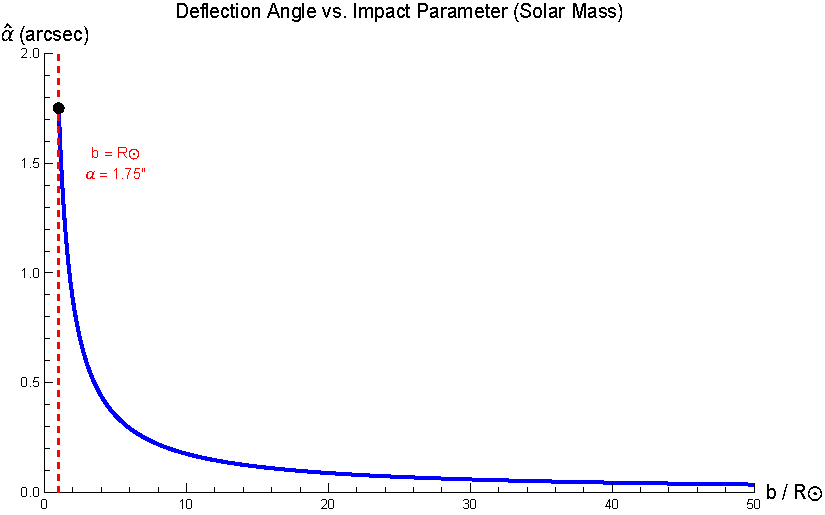
\includegraphics[width=0.75\textwidth]{../Figures/02_Light_Deflection/deflection_vs_impact.pdf}
    \caption{Deflection angle $\alphahat$ as a function of impact
    parameter~$b$ for a solar-mass lens, shown in arcseconds.  The
    deflection falls as $1/b$.  The vertical dashed line marks the solar
    radius ($b = \Rsun$) where $\alphahat = 1.75''$.  Generated by
    \texttt{deflection\_angle.wl}.}
    \label{fig:deflection_vs_impact}
\end{figure}

\begin{exercise}
\label{ex:numerical_deflections}
Compute the deflection angle for light grazing the surface of:
\begin{enumerate}[label=(\alph*)]
    \item The Sun ($M = 1.989 \times 10^{30}$~kg,
          $R = 6.957 \times 10^{8}$~m): verify $\alphahat = 1.75''$.
    \item Jupiter ($M = 1.898 \times 10^{27}$~kg,
          $R = 7.149 \times 10^{7}$~m).
    \item A $10^{12}\,\Msun$ galaxy with effective radius
          $R_e = 10$~kpc, using $b = R_e$.
          Express the result in arcseconds.
\end{enumerate}
\end{exercise}


% =====================================================================
\section{Deflection by Galaxies}
\label{sec:deflection_galaxies}

The astrophysical power of gravitational lensing comes from the fact that
the deflection angles produced by \textit{galaxies} are of order
arcseconds --- large enough to produce multiple images, arcs, and rings
that are observable with ground-based and space-based telescopes.

For a galaxy of mass $M = 10^{12}\,\Msun$ with a typical scale of
$b \sim 10$~kpc~$\approx 3.09 \times 10^{20}$~m:
\begin{equation}
    \alphahat \sim \frac{4\Gnewton M}{\speedoflight^2\, b}
    = \frac{4 \times 6.674 \times 10^{-11} \times 10^{12} \times 1.989 \times 10^{30}}
          {(2.998 \times 10^{8})^2 \times 3.09 \times 10^{20}}
    \approx 3.9''
    \label{eq:deflection_galaxy}
\end{equation}
The corresponding Einstein radius (which we will derive properly in
Module~4) is of order $\sim 1''$, depending on the distance configuration.

\begin{remark}
The Einstein radius $\thetaE$ for a point mass lens at cosmological
distances is:
\begin{equation}
    \thetaE = \sqrt{\frac{4\Gnewton M}{\speedoflight^2}
    \frac{\Dds}{\Dd\,\Ds}} \,.
    \label{eq:einstein_radius_deflection}
\end{equation}
For a $10^{12}\,\Msun$ galaxy at $z_d \sim 0.3$ with a source at
$z_s \sim 1$, this gives $\thetaE \sim 1''$.  Multiple images form
whenever the source lies within $\sim \thetaE$ of the optical axis ---
this is the regime of \textbf{strong gravitational lensing}.  We will
develop this quantitatively in Modules~4--5.
\end{remark}


% =====================================================================
\section{Exact vs.\ Weak-Field Deflection}
\label{sec:exact_vs_approx}

The weak-field formula $\alphahat = 4m/b$ is a first-order approximation
valid when $b \gg \RS$.  For photons passing closer to the mass, higher-order
corrections become important.  The \textit{exact} deflection angle is
obtained by evaluating the integral~\eqref{eq:delta_phi_u2} numerically
(or using elliptic integrals), without the weak-field expansion.

\begin{figure}[ht]
    \centering
    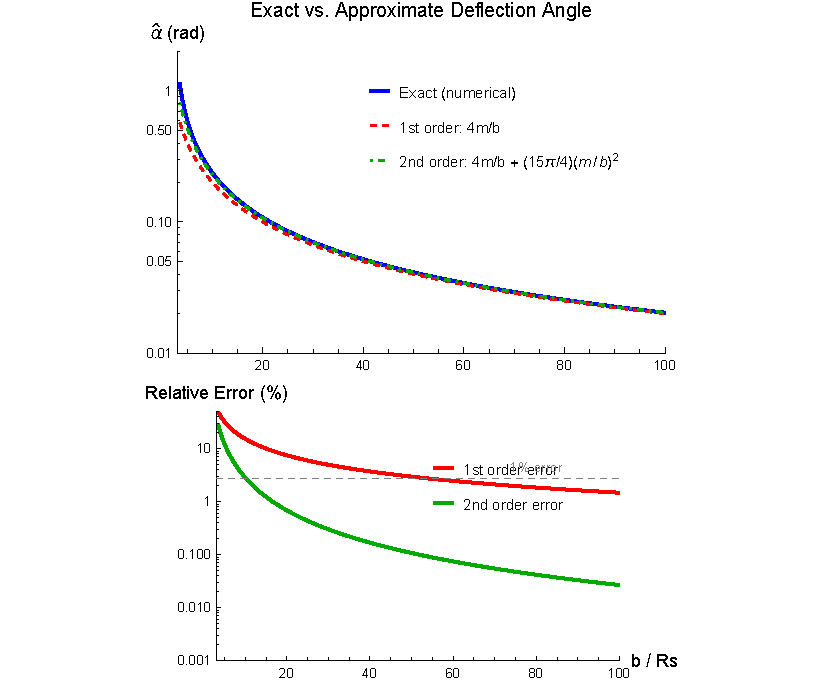
\includegraphics[width=0.75\textwidth]{../Figures/02_Light_Deflection/exact_vs_approx.pdf}
    \caption{Comparison of the exact deflection angle (solid blue, from
    numerical integration) and the weak-field approximations
    $\alphahat = 4m/b$ (dashed red, first order) and including the
    second-order correction (dot-dashed green), as a function of $b/\RS$.
    The lower panel shows the relative error.  The first-order
    approximation has $\sim 15\%$ error at $b = 10\,\RS$ and reaches
    $1\%$ accuracy only for $b \gtrsim 150\,\RS$.  At the photon sphere
    $b = 3\sqrt{3}\,\RS/2$, the exact deflection diverges (the photon
    orbits the mass).  Generated by \texttt{deflection\_angle.wl}.}
    \label{fig:exact_vs_approx}
\end{figure}

The second-order correction has been computed by several authors; the
result is (see, e.g., Keeton \& Petters 2006):
\begin{equation}
    \alphahat = \frac{4m}{b} + \frac{15\pi}{4}\left(\frac{m}{b}\right)^2
    + \order{m/b}^3 \,.
    \label{eq:deflection_second_order}
\end{equation}
The critical impact parameter below which the photon is captured (i.e.,
spirals into the mass) is $b_{\mathrm{crit}} = 3\sqrt{3}\,m =
3\sqrt{3}\,\RS/2$.  This corresponds to the photon sphere derived in
Module~1d.

\begin{exercise}
\label{ex:exact_vs_approx}
For a photon passing a Schwarzschild black hole at impact parameter
$b = 10\,\RS$:
\begin{enumerate}[label=(\alph*)]
    \item Evaluate the deflection integral~\eqref{eq:delta_phi_u2}
          numerically to obtain the exact deflection angle.
    \item Compare with the weak-field approximation
          $\alphahat = 4m/b = 0.2$~rad.  What is the relative error?
    \item Repeat for several values of $b/\RS$ from $5$ to $100$.  At what
          $b/\RS$ does the weak-field approximation first achieve 1\%
          accuracy?
\end{enumerate}
\textit{Use the Mathematica script}
\mathlink{02_Light_Deflection/deflection_angle.wl}{deflection\_angle.wl}
\textit{to verify your results.}
\end{exercise}


% =====================================================================
\section{Summary}
\label{sec:deflection_summary}

\begin{itemize}
    \item Light follows null geodesics in Schwarzschild spacetime.  The
          orbit equation~\eqref{eq:photon_orbit_eq} reduces to an integral
          for the total azimuthal angle change~$\Delta\phi$.

    \item \textbf{Newtonian prediction} (Soldner, 1801):
          $\alphahat_{\mathrm{Newton}} = 2\Gnewton M /
          (\speedoflight^2 b)$.  This accounts for only the
          \textit{temporal} curvature of spacetime.

    \item \textbf{GR prediction} (Einstein, 1915):
          $\alphahat = 4\Gnewton M / (\speedoflight^2 b)$.
          The factor of~$2$ enhancement comes from \textit{spatial}
          curvature, which contributes equally to the deflection.

    \item \textbf{Shapiro time delay:} A gravitational field causes an
          excess travel time $\Delta T$ with geometric and gravitational
          components.  This is connected to the Fermat potential
          (Module~6).

    \item \textbf{Solar deflection:} $\alphahat_\odot = 1.75''$, confirmed
          by Eddington (1919) and modern measurements to $< 0.01\%$.

    \item \textbf{Galaxy-scale lensing:} $\alphahat \sim 1''$--$4''$
          for $\sim 10^{12}\,\Msun$ galaxies at $b \sim 10$~kpc,
          producing multiple images, arcs, and Einstein rings in strong
          lensing.

    \item The weak-field approximation $\alphahat = 4m/b$ converges
          slowly; the error is $\sim 15\%$ at $b = 10\,\RS$ and drops
          below $1\%$ only for $b \gtrsim 150\,\RS$.  The exact
          deflection diverges at the photon sphere ($b_{\mathrm{crit}} =
          3\sqrt{3}\,\RS/2$).
\end{itemize}


% =====================================================================
\section{Problems}
\label{sec:deflection_problems}

\begin{exercise}
\label{ex:soldner_full}
\textbf{(Soldner's Newtonian deflection.)}
Derive the Newtonian deflection angle for a ``corpuscle of light''
traveling at speed $\speedoflight$ past a mass $M$ at impact parameter $b$.
\begin{enumerate}[label=(\alph*)]
    \item Write the Newtonian orbit equation and identify the semi-latus
          rectum $p$ and eccentricity $e$ in terms of $b$, $M$, $\Gnewton$,
          and $\speedoflight$.
    \item Show that the deflection angle is
          $\alphahat_{\mathrm{Newton}} = 2\Gnewton M /
          (\speedoflight^2 b)$ in the weak-field limit.
    \item Compute the Newtonian prediction for the solar deflection.  You
          should get $0.875''$.
\end{enumerate}
\end{exercise}

\begin{exercise}
\label{ex:factor_of_two}
\textbf{(The factor of 2: GR vs.\ Newton.)}
\begin{enumerate}[label=(\alph*)]
    \item Starting from the result $\Delta\phi = \pi + 4m/r_0$, show that
          the GR deflection angle is $\alphahat = 4\Gnewton M /
          (\speedoflight^2 b)$.
    \item The Newtonian result uses only $g_{tt} \approx -(1 - 2\Phi/
          \speedoflight^2)$ where $\Phi = -\Gnewton M/r$.  In GR, the
          spatial part of the Schwarzschild metric also curves:
          $g_{rr} \approx 1 + 2\Gnewton M/(\speedoflight^2 r)$.
          Argue qualitatively (or using the isotropic form of the metric)
          that the spatial curvature contributes an \textit{equal} amount
          of deflection, doubling the Newtonian result.
\end{enumerate}
\end{exercise}

\begin{exercise}
\label{ex:deflections_numerical}
\textbf{(Deflection for Sun, Jupiter, and galaxy.)}
Compute $\alphahat$ for:
\begin{enumerate}[label=(\alph*)]
    \item Light grazing the Sun: $M = 1.989 \times 10^{30}$~kg,
          $b = \Rsun = 6.957 \times 10^{8}$~m.
    \item Light grazing Jupiter: $M = 1.898 \times 10^{27}$~kg,
          $b = R_J = 7.149 \times 10^{7}$~m.
    \item A $10^{12}\,\Msun$ galaxy at $b = 10$~kpc.
\end{enumerate}
Express all answers in arcseconds.  Verify with
\solnlink{02_Light_Deflection/problems\_02.wl}{problems\_02.wl}.
\end{exercise}

\begin{exercise}
\label{ex:shapiro_radar}
\textbf{(Shapiro time delay for radar echoes.)}
A radar signal is sent from Earth, passes near the Sun at closest approach
$r_0$, bounces off Mercury, and returns.
\begin{enumerate}[label=(\alph*)]
    \item Using eq.~\eqref{eq:travel_time_expanded}, show that the excess
          round-trip time is
          \begin{equation*}
              \Delta T \approx
              \frac{4\Gnewton \Msun}{\speedoflight^3}
              \left[\ln\!\left(\frac{4\, R_\oplus\, R_{\mathrm{Merc}}}{r_0^2}
              \right) + 1\right]
          \end{equation*}
          where $R_\oplus = 1.496 \times 10^{11}$~m and
          $R_{\mathrm{Merc}} = 5.79 \times 10^{10}$~m are the
          Earth--Sun and Mercury--Sun distances.
    \item For $r_0 = \Rsun$, compute $\Delta T$ in microseconds.
    \item Shapiro's 1964 measurement using the Haystack radar gave
          $\Delta T = 200 \pm 20~\mu$s.  Is this consistent?
\end{enumerate}
\end{exercise}

\begin{exercise}
\label{ex:strong_field}
\textbf{(Exact vs.\ weak-field deflection.)}
For a photon passing a Schwarzschild mass at impact parameter $b = 10\,\RS$:
\begin{enumerate}[label=(\alph*)]
    \item Evaluate the exact deflection angle by numerically integrating
          eq.~\eqref{eq:delta_phi_u2}.
    \item Compare with the first-order approximation
          $\alphahat_1 = 4m/b$ and the second-order approximation
          $\alphahat_2 = 4m/b + (15\pi/4)(m/b)^2$.
    \item Tabulate the relative error of $\alphahat_1$ and $\alphahat_2$
          for $b/\RS = 5, 10, 20, 50, 100$.
    \item At what value of $b/\RS$ does the first-order approximation
          first achieve $1\%$ accuracy?
\end{enumerate}
\textit{Use}
\mathlink{02_Light_Deflection/deflection_angle.wl}{deflection\_angle.wl}
\textit{to generate and verify your results.}
\end{exercise}
